% ============================================================
% Final Project Presentation
% Project 11: Fake News & Misinformation Detection System
% Course: CSC15012 - Applications of NLP in Industry
% Student: Le Dinh Minh Quan - 23127460 - 23CNTThuc
% Template based on Madrid + seahorse (Overleaf Beamer)
% ============================================================

\documentclass[10pt,aspectratio=169]{beamer}

\mode<presentation>
{
  \usetheme{Madrid}
  \usecolortheme{seahorse}
  \usefonttheme{default}
  \setbeamertemplate{navigation symbols}{}
  \setbeamertemplate{caption}[numbered]
  \setbeamertemplate{footline}[frame number]
}

% ---- Packages ----
\usepackage[english]{babel}
\usepackage[utf8]{inputenc}
\usepackage{amsmath}
\usepackage{graphicx}
\usepackage{booktabs}
\usepackage{xcolor}
\usepackage{hyperref}
\usepackage{xurl}
\usepackage{tikz}
\usepackage{pgfplots}
\pgfplotsset{compat=1.18}
\usetikzlibrary{shapes.geometric, arrows.meta, positioning, fit, backgrounds, shadows}
\usepackage{listings}
\lstset{
  basicstyle=\ttfamily\scriptsize,
  breaklines=true,
  frame=single,
  backgroundcolor=\color{gray!10},
  keywordstyle=\color{blue},
  commentstyle=\color{green!60!black},
  stringstyle=\color{red!70!black},
  showstringspaces=false,
  tabsize=2
}

% ---- HCMUS LOGO ----
% Upload logo_hcmus.png to Overleaf to display the logo (top-right of every slide).
% If the file is missing, no logo is shown (no error).
\IfFileExists{logo_hcmus.png}{\logo{\includegraphics[height=0.7cm]{logo_hcmus.png}}}{}

% ---- TITLE METADATA ----
\title[Project 11: Fake News Detection]{Project 11: Fake News \& Misinformation Detection System}
\subtitle{A Trainable Credibility Classifier wrapped by an Agentic, Evidence-Grounded Fact-Check}
\author[Le Dinh Minh Quan]{Le Dinh Minh Quan \\ \small ID: 23127460 -- Class: 23CNTThuc}
\institute[HCMUS]{Vietnam National University Ho Chi Minh City \\ University of Science -- Faculty of Information Technology \\ \small Course: CSC15012 -- Applications of NLP in Industry}
\date{2026}

\begin{document}

% ============================================================
% SLIDE 1: TITLE
% ============================================================
\begin{frame}
  \titlepage
\end{frame}

% ============================================================
% SLIDE 2: OUTLINE
% ============================================================
\begin{frame}{Outline}
\begin{columns}[T]
\begin{column}{0.5\textwidth}
\begin{enumerate}
  \item Business Problem \& Motivation
  \item Proposed NLP Solution \& Success Metrics
  \item System Architecture
  \item Repository \& Tech Stack
  \item Data \& Licenses
  \item Training / Autopilot Workflow
  \item Evaluation Results (offline) + chart
  \item The Offline-vs-Colab Story
\end{enumerate}
\end{column}
\begin{column}{0.5\textwidth}
\begin{enumerate}
  \setcounter{enumi}{8}
  \item Agentic AI Component (5 decisions)
  \item Example Interaction Trace
  \item Deployment (API / UI / CLI / Docker)
  \item Ethics, Privacy \& Robustness
  \item Monitoring \& Continual Learning
  \item Key Takeaways \& Future Work
  \item Resources \& Thank You
\end{enumerate}
\end{column}
\end{columns}
\end{frame}

% ============================================================
% SLIDE 3: BUSINESS PROBLEM & MOTIVATION
% ============================================================
\begin{frame}{1. Business Problem \& Motivation}
\begin{block}{Context}
Online claims and news far exceed human fact-checking capacity. Misinformation spreads fast -- but the wrong automated response (auto-removal) chills free speech and silences legitimate journalism.
\end{block}

\begin{columns}[T]
\begin{column}{0.5\textwidth}
\textbf{Pain points}
\begin{itemize}
  \item Volume $\gg$ reviewer capacity
  \item False positives (real flagged fake) = the high-cost error
  \item Verdicts must be auditable (evidence)
  \item Brittle keyword filters can't judge evidence
\end{itemize}
\end{column}
\begin{column}{0.5\textwidth}
\textbf{Stakeholders}
\begin{itemize}
  \item Journalists / fact-checkers
  \item Trust \& Safety / moderators
  \item Newsroom editors / researchers
  \item End readers (secondary)
\end{itemize}
\end{column}
\end{columns}

\vspace{0.15cm}
\centering\small \textbf{Non-negotiable}: the tool \emph{flags for human review}, always shows its evidence, and \textbf{never auto-removes or censors.}
\end{frame}

% ============================================================
% SLIDE 4: PROPOSED NLP SOLUTION + SUCCESS METRICS
% ============================================================
\begin{frame}{2. Proposed NLP Solution \& Success Metrics}
\begin{block}{Solution -- two clearly separated signals}
A \textbf{trainable transformer classifier} (fast credibility \emph{prior} $P(\text{fake})$) wrapped by an \textbf{agentic, evidence-grounded fact-check}: extract claim $\rightarrow$ retrieve $\rightarrow$ stance/NLI $\rightarrow$ aggregate verdict + citations $\rightarrow$ \textbf{abstain} when uncertain.
\end{block}

\begin{table}[h]
\centering\small
\begin{tabular}{lll}
\toprule
\textbf{Type} & \textbf{Metric} & \textbf{Framing} \\
\midrule
Business & Reviewer throughput / flag precision & Triage the firehose to humans \\
Business & Evidence-grounding rate & 100\% non-abstained verdicts cite evidence \\
Technical & Macro-F1 (headline) & In-domain \textbf{and} cross-domain (honest) \\
Technical & Calibration (ECE) & Over-confidence can silence real news \\
Technical & Label acc.\ + recall@k + selective acc. & FEVER-style + abstain quality \\
\bottomrule
\end{tabular}
\end{table}

\small \textbf{Macro-F1} is the headline number; \textbf{the cross-domain drop is the honest classifier metric} and is itself an ethics metric. The classifier prior and the evidence verdict are reported \textbf{separately}.
\end{frame}

% ============================================================
% SLIDE 5: SYSTEM ARCHITECTURE (TikZ)
% ============================================================
\begin{frame}{3. System Architecture (single app, two signals)}
\centering
\resizebox{\linewidth}{!}{%
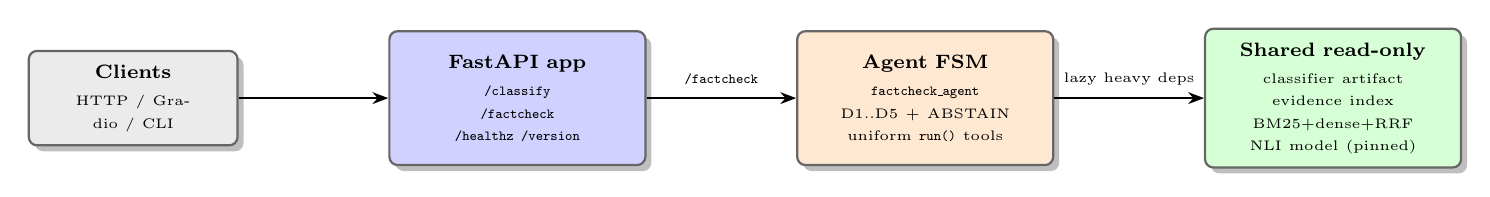
\begin{tikzpicture}[
  node distance=0.8cm and 1.9cm,
  box/.style={rectangle, draw=black!60, rounded corners=3pt, thick,
              text width=2.9cm, minimum height=1.7cm, align=center,
              inner sep=5pt, font=\scriptsize, drop shadow},
  clientbox/.style={box, fill=gray!16, text width=2.3cm, minimum height=1.1cm},
  apibox/.style={box, fill=blue!18},
  agentbox/.style={box, fill=orange!18},
  statebox/.style={box, fill=green!16},
  arrow/.style={-{Stealth[length=2mm]}, thick}
]
\node[clientbox] (cli) {\textbf{Clients}\\[2pt]{\tiny HTTP / Gradio / CLI}};
\node[apibox, right=of cli] (api) {%
  \textbf{FastAPI app}\\[2pt]
  {\tiny \texttt{/classify}}\\
  {\tiny \texttt{/factcheck}}\\
  {\tiny \texttt{/healthz} \texttt{/version}}
};
\node[agentbox, right=of api] (agent) {%
  \textbf{Agent FSM}\\[2pt]
  {\tiny \texttt{factcheck\_agent}}\\
  {\tiny D1..D5 + ABSTAIN}\\
  {\tiny uniform \texttt{run()} tools}
};
\node[statebox, right=of agent] (state) {%
  \textbf{Shared read-only}\\[2pt]
  {\tiny classifier artifact}\\
  {\tiny evidence index}\\
  {\tiny BM25+dense+RRF}\\
  {\tiny NLI model (pinned)}
};
\draw[arrow] (cli.east) -- (api.west);
\draw[arrow] (api.east) -- node[above=1pt, font=\tiny, midway] {\texttt{/factcheck}} (agent.west);
\draw[arrow] (agent.east) -- node[above=1pt, font=\tiny, midway] {lazy heavy deps} (state.west);
\end{tikzpicture}%
}

\vspace{0.2cm}
\scriptsize Cheap classifier prior runs per request; the heavier retrieval+NLI fact-check is \textbf{gated behind \texttt{/factcheck}}. Heavy imports happen inside each tool's \texttt{run()} -- with \textbf{no torch} the service still boots on the TF-IDF + BM25 path.
\end{frame}

% ============================================================
% SLIDE 6: REPOSITORY & TECH STACK
% ============================================================
\begin{frame}[fragile]{4. Repository Structure \& Tech Stack}
\begin{columns}[T]
\begin{column}{0.55\textwidth}
\textbf{GitHub repo} (public, MIT) \\
\scriptsize \url{https://github.com/ledinhminhquan/11_Fake_News_Detection}

\vspace{0.15cm}
\begin{lstlisting}[basicstyle=\ttfamily\tiny]
src/fakenews/                 # no-torch core
|-- config.py cli.py logging_utils.py
|-- data/      samples.py (seed) dataset.py
|-- models/    classifier.py bm25.py registry
|-- factcheck/ retriever.py stance.py verdict.py
|-- agent/     state policy(D1-D5) tools
|              llm_orchestrator fakenews_agent
|-- api/       main /classify /factcheck ui(Gradio)
|-- training/  train_classifier baseline eval tune
|-- analysis/ autoreport/ monitoring/ grading/
configs/ docs/ tests/ notebooks/ app/ deploy/
Dockerfile docker-compose.yml README.md
\end{lstlisting}
\end{column}
\begin{column}{0.45\textwidth}
\textbf{Tech stack}
\begin{itemize}\small
  \item Python 3.12, Git + GitHub (MIT)
  \item Core: numpy/pandas/sklearn/\texttt{rank\_bm25} (\textbf{no torch})
  \item \texttt{[ml]}: PyTorch, Transformers, sentence-transformers (lazy)
  \item Classifier: \textbf{distilbert} / deberta-v3 / ModernBERT
  \item Baselines: majority, TF-IDF+LogReg, zero-shot
  \item Stance: \textbf{DeBERTa-v3-mnli-fever-anli} (MIT)
  \item Retrieval: BM25 + MiniLM + RRF + rerank
  \item FastAPI + Gradio + Docker / HF Space
  \item Colab autopilot (auto-profiles H100/A100/L4/T4)
\end{itemize}
\end{column}
\end{columns}
\end{frame}

% ============================================================
% SLIDE 7: DATA & LICENSES
% ============================================================
\begin{frame}{5. Data \& Licenses (hygiene is explicit)}
\begin{columns}[T]
\begin{column}{0.52\textwidth}
\textbf{Classifier data}
\begin{itemize}\scriptsize
  \item \texttt{GonzaloA/fake\_news} -- PRIMARY binary, license \textbf{unknown (FLAG)}
  \item \texttt{chengxuphd/liar2} -- Apache, 6-way credibility
  \item \texttt{mohammadjavadpirhadi/...} -- MIT-clean alt
  \item \texttt{LittleFish-Coder/...GossipCop} -- Apache, \textbf{cross-domain eval}
\end{itemize}
\textbf{Fact-check data}
\begin{itemize}\scriptsize
  \item \texttt{fever/*}, \texttt{copenlu/*}, \texttt{BeIR/*} -- cc-by-sa \textbf{(copyleft FLAG)}
  \item \texttt{allenai/scifact} -- cc-by-nc \textbf{(NON-COMMERCIAL -- avoided)}
\end{itemize}
\end{column}
\begin{column}{0.48\textwidth}
\textbf{Polarity gotcha (normalize on load)}
\begin{itemize}\scriptsize
  \item Internal: \textbf{0=real, 1=fake}
  \item GonzaloA native 0=fake; LittleFish 0=real; mrm8488 1=fake
  \item Every loader applies a per-source \texttt{label\_map}
\end{itemize}
\textbf{Offline synthetic spine}
\begin{itemize}\scriptsize
  \item \textbf{40} seed items + \textbf{16} evidence + \textbf{8} gold claims
  \item Runs the \emph{whole} pipeline, no network, no torch
\end{itemize}
\textbf{Anti-leakage}
\begin{itemize}\scriptsize
  \item Strip source/dateline boilerplate; dedup; drop LIAR metadata
  \item FakeNewsNet raw is a crawler $\rightarrow$ excluded from CI
\end{itemize}
\end{column}
\end{columns}
\end{frame}

% ============================================================
% SLIDE 8: TRAINING / AUTOPILOT WORKFLOW
% ============================================================
\begin{frame}{6. Training / Autopilot Workflow}
\centering
\begin{tikzpicture}[
  node distance=0.16cm,
  step/.style={rectangle, draw=black!60, rounded corners=2pt, thick,
              minimum width=11.6cm, minimum height=0.52cm, align=center, font=\scriptsize},
  setup/.style={step, fill=gray!15},
  train/.style={step, fill=orange!15},
  eval/.style={step, fill=blue!15},
  deploy/.style={step, fill=green!15},
  arrow/.style={-{Stealth[length=1.8mm]}, thick}
]
\node[setup] (s1) {\textbf{1. Setup}: mount Drive, install Colab-safe deps, \textbf{auto-profile GPU} (H100/A100/L4 bf16 $\cdot$ T4 fp16)};
\node[setup, below=of s1] (s2) {\textbf{2. Data}: GonzaloA / LIAR2; per-source \texttt{label\_map}; strip boilerplate; dedup};
\node[train, below=of s2] (s3) {\textbf{3. Baseline}: TF-IDF + LogReg floor (the number to beat)};
\node[train, below=of s3] (s4) {\textbf{4. Fine-tune}: transformer $\leq$3 epochs + early stop; class weights; \textbf{temperature-scaling}};
\node[eval, below=of s4] (s5) {\textbf{5. Eval}: macro-F1 / per-class / ROC-AUC / ECE + \textbf{cross-domain} GonzaloA$\rightarrow$GossipCop drop};
\node[eval, below=of s5] (s6) {\textbf{6. Fact-check eval}: retrieve $\rightarrow$ NLI stance $\rightarrow$ verdict; label acc + recall@k + risk--coverage};
\node[deploy, below=of s6] (s7) {\textbf{7. Auto-gen} report PDF + slides PPTX (confusion matrix, verdict distribution)};
\node[deploy, below=of s7] (s8) {\textbf{8. Self-grade}: \texttt{fakenews grade} runs the rubric checklist; bundle artifacts};
\foreach \a/\b in {s1/s2,s2/s3,s3/s4,s4/s5,s5/s6,s6/s7,s7/s8}
  \draw[arrow] (\a) -- (\b);
\end{tikzpicture}

\vspace{0.12cm}
\scriptsize \textbf{One-button} Colab autopilot; also runs offline (\texttt{autopilot --no-train}) on the seed with no GPU. CI is download-free and torch-free.
\end{frame}

% ============================================================
% SLIDE 9: EVALUATION RESULTS (offline) + chart
% ============================================================
\begin{frame}{7. Evaluation Results -- Offline Seed (no torch)}
\begin{columns}[T]
\begin{column}{0.52\textwidth}
\textbf{Classifier} (40-item engineered-separable seed)
\begin{table}[h]
\centering\scriptsize
\begin{tabular}{lcccc}
\toprule
\textbf{System} & \textbf{Acc} & \textbf{F1$_M$} & \textbf{AUC} & \textbf{ECE} \\
\midrule
\textbf{TF-IDF + LogReg} & \textbf{1.000} & \textbf{1.000} & \textbf{1.000} & \textbf{0.244} \\
Majority class & -- & 0.333 & -- & -- \\
\bottomrule
\end{tabular}
\end{table}

\textbf{Agentic fact-check} (8 gold claims)
\begin{table}[h]
\centering\scriptsize
\begin{tabular}{lcc}
\toprule
\textbf{System} & \textbf{Label acc} & \textbf{Coverage} \\
\midrule
Agentic fact-check & \textbf{1.000} & \textbf{1.000} \\
\bottomrule
\end{tabular}
\end{table}

\scriptsize Saturates \textbf{by design} (proves the metric \& FSM plumbing, \emph{not} capability). \textbf{ECE = 0.244 at 100\% accuracy} is the live demo of the over-confidence pathology $\Rightarrow$ why temperature scaling exists.
\end{column}
\begin{column}{0.48\textwidth}
\centering
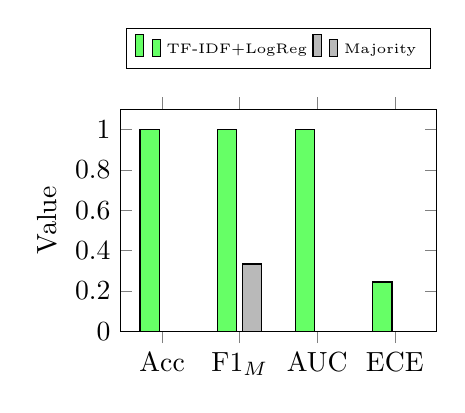
\begin{tikzpicture}
\begin{axis}[
  ybar, width=5.6cm, height=4.4cm,
  ymin=0, ymax=1.1,
  symbolic x coords={Acc, F1$_M$, AUC, ECE},
  xtick=data,
  ylabel={Value},
  legend style={font=\tiny, at={(0.5,1.18)}, anchor=south, legend columns=2},
  bar width=7pt,
  enlarge x limits=0.18,
  ytick={0,0.2,0.4,0.6,0.8,1.0}
]
\addplot[fill=green!60] coordinates {(Acc,1.0) (F1$_M$,1.0) (AUC,1.0) (ECE,0.244)};
\addplot[fill=gray!55] coordinates {(Acc,0) (F1$_M$,0.333) (AUC,0) (ECE,0)};
\legend{TF-IDF+LogReg, Majority}
\end{axis}
\end{tikzpicture}

\scriptsize Majority macro-F1 $= 0.333$ is the textbook floor (F1$=0$ on the never-predicted class).
\end{column}
\end{columns}
\end{frame}

% ============================================================
% SLIDE 10: THE OFFLINE-VS-COLAB STORY
% ============================================================
\begin{frame}{8. The Offline-vs-Colab Story (honesty)}
\begin{columns}[T]
\begin{column}{0.5\textwidth}
\textbf{Verified offline (no torch) -- proves the plumbing}
\begin{itemize}\small
  \item acc / macro-F1 / per-class / ROC-AUC / ECE all compute
  \item majority + TF-IDF baselines wired \& comparable
  \item ECE surfaces over-confidence even at 100\% acc
  \item full FSM (D1--D5) executes; support/refute/abstain reachable
  \item verbatim citations + \texttt{decisions\_trace} returned
\end{itemize}
\end{column}
\begin{column}{0.5\textwidth}
\textbf{Produced by the real Colab H100 run}
\begin{itemize}\small
  \item real classifier macro-F1 (in-domain $\approx$ 0.90)
  \item \textbf{the cross-domain drop} (GonzaloA$\rightarrow$GossipCop) -- the honest number
  \item calibrated confidences after temperature scaling
  \item FEVER label accuracy + evidence recall@k at scale
  \item abstention quality on genuinely-uncovered claims
\end{itemize}
\end{column}
\end{columns}

\vspace{0.2cm}
\centering
\small \textbf{The seed saturates by design; the Colab run produces the real, lower, honest numbers.} The cross-domain drop is the source-style-leakage signature -- itself an ethics metric.
\end{frame}

% ============================================================
% SLIDE 11: AGENTIC AI COMPONENT (5 decisions)
% ============================================================
\begin{frame}{9. Agentic AI Component (5-Decision FSM)}
\centering
\resizebox{0.96\linewidth}{!}{%
\begin{tikzpicture}[
  node distance=0.16cm,
  step/.style={rectangle, draw=black!60, rounded corners=2pt, thick,
              text width=11.6cm, minimum height=0.5cm, align=center, font=\scriptsize, inner sep=3pt},
  clf/.style={step, fill=purple!15},
  dec/.style={step, fill=red!12},
  ir/.style={step, fill=blue!15},
  nli/.style={step, fill=orange!15},
  pres/.style={step, fill=green!15},
  arrow/.style={-{Stealth[length=1.8mm]}, thick}
]
\node[dec] (a1) {\textbf{D1 Claim routing} (\textbf{reasoning}): \texttt{tokens$\leq$40}/no body $\rightarrow$ short claim; else article $\rightarrow$ extract central claim};
\node[clf, below=of a1] (a2) {\textbf{Classify} (\textbf{tool}): transformer / TF-IDF $\rightarrow$ prior $P(\text{fake})$};
\node[dec, below=of a2] (a3) {\textbf{D2 Check-worthiness gate} (\textbf{decision}): \texttt{conf$\geq$0.95} \& not-claim $\rightarrow$ skip; else retrieve};
\node[ir, below=of a3] (a4) {\textbf{Retrieve} (\textbf{tool}): BM25 + dense (MiniLM) $\rightarrow$ RRF $\rightarrow$ rerank};
\node[dec, below=of a4] (a5) {\textbf{D3 Evidence-coverage gate} (\textbf{reasoning}): \texttt{$n_{\text{rel}}\geq3$}? else widen $\leq2$ then \textbf{ABSTAIN}};
\node[nli, below=of a5] (a6) {\textbf{Stance / NLI} (\textbf{tool}): premise=evidence, hypothesis=claim $\rightarrow$ support/refute/neutral};
\node[dec, below=of a6] (a7) {\textbf{D4 Verdict gate} (\textbf{reasoning}): $S=\sum w_i s_i$, $\alpha{=}0.6$, $\theta{=}0.2 \rightarrow$ REAL/FAKE/UNVERIFIED};
\node[dec, below=of a7] (a8) {\textbf{D5 Confidence / abstain gate} (\textbf{decision}): low conf / low agreement / prior$\leftrightarrow$stance conflict $\rightarrow$ abstain};
\node[pres, below=of a8] (a9) {\textbf{Present}: label + confidence + \textbf{verbatim citations} + \texttt{decisions\_trace}};
\foreach \a/\b in {a1/a2,a2/a3,a3/a4,a4/a5,a5/a6,a6/a7,a7/a8,a8/a9}
  \draw[arrow] (\a) -- (\b);
\end{tikzpicture}%
}

\vspace{0.1cm}
\scriptsize Deterministic FSM; optional LLM brain may only \textbf{propose} legal values (never decides flow, never invents a verdict/citation). \textbf{Evidence dominates; the prior is a soft nudge.}
\end{frame}

% ============================================================
% SLIDE 12: EXAMPLE INTERACTION TRACE
% ============================================================
\begin{frame}[fragile]{10. Example Interaction (every decision fires)}
\begin{lstlisting}[basicstyle=\ttfamily\tiny]
Input: "The WHO declared that drinking bleach cures COVID-19 in 2021."

  Classify  -> label=fake, p_fake=0.88, backend=transformer
D1 ClaimExtract -> 11 tokens <= 40 -> short-claim route
   entities=[WHO, COVID-19, 2021, bleach]
D2 CheckWorthy  -> conf 0.88 < 0.95 -> do NOT skip; checkworthy=0.92 -> RETRIEVE
D3 Retrieve     -> RRF(BM25,dense) -> 4 passages rerank>=0.3; n_rel=4>=3 -> coverage_ok
   Stance/NLI   -> 3x contradiction->refute (~0.94), 1x neutral
D4 Aggregate    -> S ~ -2.7; prior agrees; |S|>theta -> verdict=FAKE/REFUTED, conf=0.91
D5 Decide       -> agreement 0.75>=0.4; conf 0.91>=0.55; no conflict -> PRESENT
Present -> label=fake, confidence=0.91,
   citations=[3 refuting WHO/fact-check passages: id+source+snippet+stance],
   rationale="Multiple authoritative sources contradict this claim; none support it.",
   abstained=false  (full ToolTrace attached)

# Counter-example: novel uncovered claim -> D3 widens twice, still n_rel<3
#   -> ABSTAIN "unverified (insufficient evidence)" -- never a guessed label
\end{lstlisting}
\scriptsize \texttt{classifier\_prior} and the evidence \texttt{verdict} are returned as \textbf{separate fields} so a reviewer sees any conflict.
\end{frame}

% ============================================================
% SLIDE 13: DEPLOYMENT
% ============================================================
\begin{frame}{11. Deployment (4 surfaces, 1 package)}
\textbf{Delivery surfaces (rubric requires only one -- we deliver four)}
\begin{itemize}\small
  \item \textbf{REST API} (FastAPI): \texttt{POST /classify}, \texttt{POST /factcheck}, \texttt{GET /healthz}, \texttt{GET /version}
  \item \textbf{Gradio UI}: two tabs (Classify / Fact-check) at \texttt{/ui}
  \item \textbf{CLI}: \texttt{fakenews classify / factcheck / serve / train-classifier / autopilot / grade}
  \item \textbf{Docker / HF Space}: CPU base + optional CUDA layer (auto-adapts H100/A100/L4/T4 $\rightarrow$ CPU/TF-IDF)
\end{itemize}

\begin{table}[h]
\centering\scriptsize
\begin{tabular}{lll}
\toprule
\textbf{Endpoint} & \textbf{Method} & \textbf{Response (key fields)} \\
\midrule
\texttt{/classify} & POST & \texttt{label, probability, prior\_fake, model\_version, backend} \\
\texttt{/factcheck} & POST & \texttt{verdict, confidence, classifier\_prior, evidence[], rationale, decisions\_trace, disclaimer, abstained} \\
\texttt{/healthz} & GET & \texttt{status, models\_loaded} \\
\texttt{/version} & GET & \texttt{classifier\_version, nli\_model, retriever, index\_built\_at, git\_sha} \\
\bottomrule
\end{tabular}
\end{table}

\small \textbf{Cold-start floor}: with no torch the service still boots on TF-IDF + BM25. \texttt{/factcheck} \textbf{always} returns evidence + \texttt{decisions\_trace}, even on abstain. \textbf{Status}: deployable; not currently hosted at a fixed live URL.
\end{frame}

% ============================================================
% SLIDE 14: ETHICS, PRIVACY & ROBUSTNESS
% ============================================================
\begin{frame}{12. Ethics, Privacy \& Robustness}
\begin{columns}[T]
\begin{column}{0.5\textwidth}
\textbf{Ethics (the centrepiece)}
\begin{itemize}\small
  \item \textbf{Flag, never censor} -- no auto-takedown anywhere
  \item False positives (real$\rightarrow$fake) = high-cost error $\Rightarrow$ optimise \texttt{real}-recall
  \item \textbf{Abstain} is first-class (\texttt{unverified} $\neq$ true)
  \item Prior vs verdict reported \textbf{separately} (conflict flag)
  \item Citations \textbf{verbatim} -- never generated/misattributed
\end{itemize}
\end{column}
\begin{column}{0.5\textwidth}
\textbf{Privacy \& Robustness}
\begin{itemize}\small
  \item Secrets via env vars; LLM brain opt-in
  \item Source-style leakage measured via cross-domain drop
  \item Adversarial paraphrase: evidence layer is robust; no ``evasion score'' (dual-use)
  \item Stale evidence: versioned/timestamped index $\rightarrow$ abstain when thin
  \item No-torch degradation: TF-IDF / BM25 / lexical stance keep the contract
\end{itemize}
\end{column}
\end{columns}

\vspace{0.15cm}
\centering\small \textbf{Limitations}: English-centric; US-politics/celebrity skew; fixed corpus. The classifier detects \emph{style}, not \emph{truth} -- the evidence layer is the trusted output.
\end{frame}

% ============================================================
% SLIDE 15: MONITORING & CONTINUAL LEARNING
% ============================================================
\begin{frame}{13. Monitoring \& Continual Learning}
\begin{columns}[T]
\begin{column}{0.5\textwidth}
\textbf{Monitoring}
\begin{itemize}\small
  \item Per-request JSONL: prior, verdict, action, backend, version stamps
  \item Drift: input-text + abstain-rate + prior$\leftrightarrow$verdict conflict-rate over time
  \item Error slices: per-source / per-topic / per-speaker (not one aggregate)
\end{itemize}
\end{column}
\begin{column}{0.5\textwidth}
\textbf{Continual learning loop}
\begin{enumerate}\small
  \item Collect reviewer overrides from the flag-for-review queue
  \item Re-label with documented provenance
  \item Retrain + re-fit temperature scaling; rebuild + re-version index
  \item Re-eval on test + \textbf{cross-domain} + fairness slices
  \item Deploy with pinned revisions (champion/challenger, easy rollback)
\end{enumerate}
\end{column}
\end{columns}

\vspace{0.2cm}
\centering
\small The \textbf{model registry + \texttt{/version}} pin classifier version, HF \emph{revision} SHAs, \texttt{index\_built\_at}, \texttt{git\_sha} into every response -- a Hub update can never silently change a verdict.
\end{frame}

% ============================================================
% SLIDE 16: KEY TAKEAWAYS & FUTURE WORK
% ============================================================
\begin{frame}{14. Key Takeaways \& Future Work}
\textbf{Key takeaways}
\begin{itemize}\small
  \item Complete end-to-end NLP system: train $\rightarrow$ eval $\rightarrow$ deploy $\rightarrow$ monitor
  \item Two separated signals: a trainable classifier \emph{prior} + an agentic, evidence-grounded \emph{verdict}
  \item 5-decision deterministic FSM (D1--D5): reasoning + tools + decisions, with \textbf{abstain} first-class
  \item Verified offline (no torch): classifier acc/F1/AUC $=1.0$, \textbf{ECE $=0.244$} (over-confidence demo); fact-check label acc $=1.0$, coverage $=1.0$
  \item Honesty built in: the \textbf{cross-domain drop} is the real classifier metric; \textbf{flag, never censor}
  \item Deployable across REST API, Gradio UI, CLI and Docker/Space; no-torch cold-start floor
\end{itemize}

\textbf{Future work}
\begin{enumerate}\small
  \item Active learning from the human-review queue
  \item Optional FEVER-fine-tuned stance head (with share-alike attribution)
  \item Larger backbones (ModernBERT-large) + more languages
  \item Token-level explainability (SHAP / LIME / Integrated Gradients)
  \item Drift dashboard + champion/challenger A/B testing
\end{enumerate}
\end{frame}

% ============================================================
% SLIDE 17: RESOURCES & THANK YOU (Final slide)
% ============================================================
\begin{frame}{15. Project Resources \& Thank You}
\begin{block}{Source code (public, MIT)}
\centering
\large \textbf{\url{https://github.com/ledinhminhquan/11_Fake_News_Detection}}
\end{block}

\textbf{Resources}
\begin{itemize}\small
  \item \textbf{GitHub repo}: \scriptsize\url{https://github.com/ledinhminhquan/11_Fake_News_Detection}
  \item \textbf{Reference}: KaiDMML/FakeNewsNet -- \scriptsize\url{https://github.com/KaiDMML/FakeNewsNet}
  \item \textbf{Deployable surfaces}: FastAPI \texttt{/classify}+\texttt{/factcheck}, Gradio UI, \texttt{fakenews} CLI, Docker / HF Space, Colab H100 autopilot notebook
\end{itemize}

\vspace{0.3cm}
\centering
\Large\textbf{Thank you for your attention!}\\[0.2cm]
\normalsize Le Dinh Minh Quan -- 23127460 -- 23CNTThuc \\
\small CSC15012 -- Applications of NLP in Industry -- 2026
\end{frame}

\end{document}
